%!TEX root = Tesi__Simone_Mariotti.tex
\chapter{Implementazione}
\fancyhead[R]{\bfseries Implementazione} 	
\fancyfoot[C]{\thepage }
Il successivo diagramma descrive in generale il processo che: preso un frame e un messaggio
di Arduino restituisce una risposta generata dalla logica dell'app.
\begin{figure}[H] \center
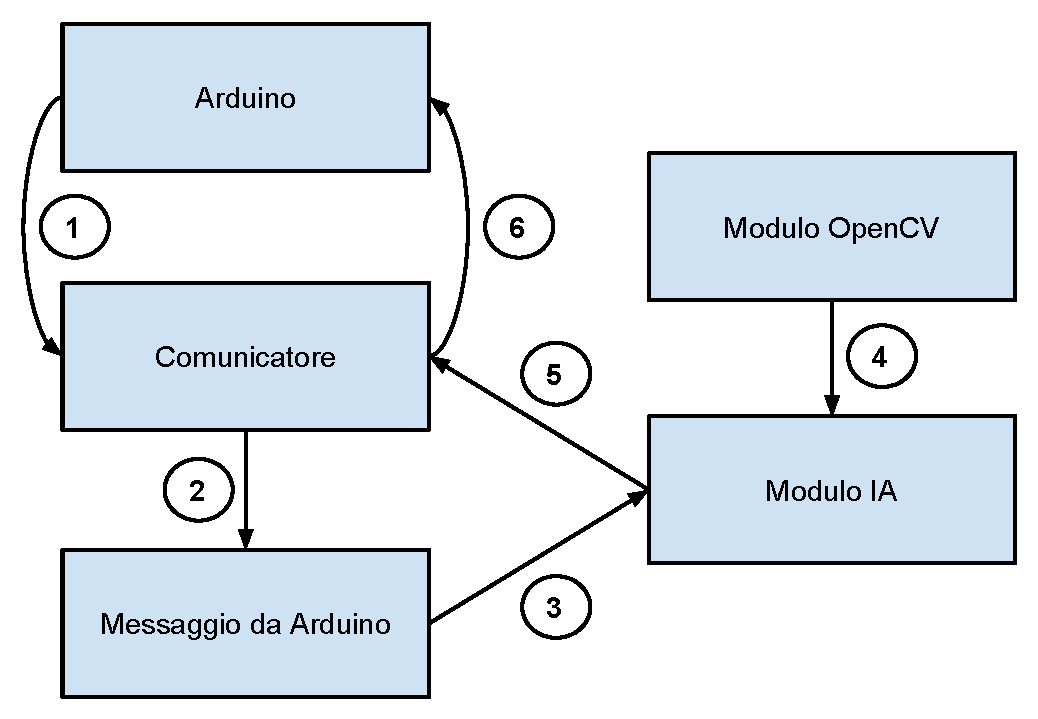
\includegraphics[width=\textwidth]{immagini/schema_processo_new.pdf}
\caption{Processo decisionale del sistema} 
\end{figure}
Le fasi principali sono:
\begin{enumerate}
\item ricezione messaggio da Arduino.
\item salvataggio e decodifica del messaggio.
\item lettura del messaggio da parte del modulo di IA\footnote{Intelligenza Artificiale}.
\item acquisizione dell'obbiettivo dall'ambiente.
\item accodamento per la trasmissione del comando elaborato dal'IA.
\item invio del comando ad Arduino.
\end{enumerate}




È definito ``agente'' una qualunque entità in grado di percepire l'ambiente
circostante attraverso dei sensori e di eseguire delle azioni attraverso degli
attuatori. Nel campo dell'intelligenza artificiale è definito intelligente quel-
l'agente che fa la cosa giusta al momento giusto. Il compito dell'agente è
quello di stabilire una sequenza di azioni che portano al raggiungimento di
uno stato obiettivo.\cite{agente}
\section {Android}
L'app per Android è stata sviluppata avendo come priorità la modularità. E' 
infatti molto semplice cambiare totalmente il comportamento dell'agente o la 
codifica dei messaggi sostituendo o modificando una singola classe senza 
coinvolgere il resto del codice.\\
La modularizzazione a grana più grossa è a livello di pacchetto\footnote{Un contenitore 
che racchiude classi che svolgono compitini affini}. Ci sono tre pacchetti,
ognuno con un compito preciso, \textbf{logic}, \textbf{messaging} e \textbf{opencv}.
\begin{figure}[H] \center
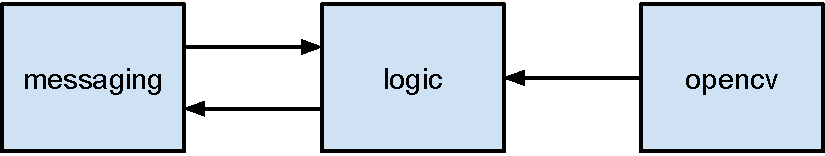
\includegraphics[width=\textwidth]{immagini/interconnessione_pacchetti.pdf}
\caption{Schema di interconnessione dei pacchetti} 
\end{figure}

\subsection {Il pacchetto \textit{opencv}}
Il pacchetto \textbf{opencv} è costituito di due sole classi. Si occupa di analizzare 
i frame proveniente dalla camera alla ricerca dell'obbiettivo, comunica poi la posizione 
dell'obbiettivo o l'assenza dello stesso alla classe RobotLogic del pacchetto 
\textbf{logic}.
\subsubsection{La classe \emph{ColorBlobDetector}}
\emph{ColorBlobDetector} è la classe che effettivamente cerca l'obbiettivo nei
frame proveniente dalla camera. L'obbiettivo gli viene fornito da RobotActivity 
tramite \emph{setTargetHsvColor()} nel momento in cui l'utente lo indica 
sull'interfaccia utente. I colori in OpenCV vengono rappresentati con un tipo di dato interno
detto Scalar che può essere assimilato ad un array. Il metodo che esegue 
l'operazione di ricerca è \emph{process()}. Per prima cosa converte lo schema di 
colori del frame sotto analisi da RGBa\footnote{Ogni colore è rappresentato da 
quattro valori compresi tra 0 e 255 per le immagini CV\_8U, cioè le immagini dove 
i colori sono memorizzati in un byte. I quattro canali sono R (red), G (green), 
B (blue) e a (alpha) }. a HSV\footnote{Ogni colore è rappresentato da quattro 
valori compresi tra 0 e 255 per le immagini CV\_8U, cioè le immagini dove 
i colori sono memorizzati in un byte. I quattro canali sono H (hue), S (saturation), 
V (value) e  a (alpha)} e filtra l'immagine in modo che rimangano solo 
i pixel che hanno un colore che si trova entro un certo intorno del colore cercato.
Usa poi la funzione fornita da OpenCV \emph{findContours()} che cerca i contorni delle
zone con il colore di nostro interesse e li restituisce come una un ArrayList di MatOfPoint;
MatOfPoint è un tipo di dato di OpenCV che è usato per memorizzare una quantità variabile
di punti che sono in relazione tra di loro, in questo caso dei punti che formano un contorno.
In seguito cerca il contorno che ha area maggiore e scarta tutti quelli che sono più piccoli 
del limite impostato ad un un'ordine di grandezza in meno. I contorni rimasti 
saranno quelli analizzati da TargetSearch.


\subsubsection{La classe \emph{TargetSearch}}
Questa classe per prima cosa invoca \emph{process()} di ColorBlobDetector passandogli
il frame da analizzare e raccoglie i risultati tramite \emph{getContours()} che restituisce 
i contorni individuati da \emph{process()}.\\
Scorre poi uno ad uno i contorni così ricevuti e trova per ognuno un ``bounding rectangle'', 
cioè il rettangolo di area minima che contiene per interno il contorno corrente, 
scartando tutti i rettangoli minori di un certo valore e mantenendo un riferimento 
a quello di area maggiore trovato fino a quel momento. I rettangoli saranno tutti colorati di blu
 tranne quello di area maggiore che sarà colorato di rosso. Sarà proprio questo 
 rettangolo il nostro obbiettivo.\\
 Fornisce un feedback all'utente sul colore scelto e la gamma di colori simili 
 che sono stati cercati.\\
 Solo tre dati forniti da questa classe servono alla RobotLogic per valutare l'azione 
 da intraprendere e sono:
 la posizione dell'obbiettivo, la larghezza del frame e il bounding rectangle 
 che racchiude l'obbiettivo.\\
 Le posizioni sono sempre riferite all'asse x in quanto l'agente non 
 ha capacità di movimento sull'asse y e possono essere:
 \begin{itemize}
	\item TARGET\_POSITION\_LEFT: il centro dell'obbiettivo si trova a sinistra del centro del frame. 
	\item TARGET\_POSITION\_RIGHT: il centro dell'obbiettivo si trova a destra del centro del frame. 
	\item TARGET\_POSITION\_FRONT: il centro dell'obbiettivo e il centro del frame coincidono. 
	\item TARGET\_POSITION\_NONE: l'obbiettivo non è visibile.
\end{itemize}
Comanda ad UpdateDirection del pacchetto \textbf{logic} di mostrare le informazioni 
corrispondenti alla posizione dell'obbiettivo.

\subsection{Il pacchetto \textit{messaging}}
Questo pacchetto è un modulo completamente a se stante, è così possibile cambiare il
 protocollo di comunicazione senza alterare la logica dell'agente. Le stringhe sono 
 tutte codificate e decodificate all'interno di questo pacchetto, non c'è nulla di 
 ``hard coded''\footnote{Una pratica considerata da evitare che prevede stringhe di 
 testo scritte direttamente nel codice}.
 \\ Nel nostro caso i messaggi sono formati da tre interi da un byte, così che il 
 range possibile è 0-255, separati da virgole.
 I messaggi diretti da Arduino ad Android hanno questa forma:
 \begin{center}
 \textbf{MessageType,Message,Data}
 \end{center}
 dove MessageType può assumere due valori: INFO, indica che il messaggio trasporta un
 dato informativo, o STATE, indica che il messaggio comunica lo stato in cui si trova Arduino.
 \\Se il MessageType è INFO allora il Message può essere di due tipi: 
 \begin{itemize}\item DISTANCE: sulla porzione Data del messaggio sarà presente 
 la distanza del primo oggetto di fronte all'agente.
 \item TERMINATE: indica l'intenzione di Arduino di chiudere l'app Android.
 \end{itemize}
 Se il MessageType è STATE allora il Message può essere di quattro tipi: 
 \begin{itemize}
 	\item IDLE: l'agente non sta eseguendo alcuna azione.
 	\item SEARCHING: l'agente si sta muovendo in cerca dell'obbiettivo.
 	\item HUNTING: l'agente si sta muovendo verso l'obbiettivo.
 	\item EMERGENCY: l'agente è in emergenza, non eseguirà nessun comando fino al 
 	termine della situazione di emergenza. 
 \end{itemize}
  I messaggi diretti da Android ad Arduino hanno invece questa forma:
 \begin{center}
 \textbf{Command,Parameter1,Parameter2}
 \end{center}
 Command identifica l'azione da eseguire, Parameter1 e Parameter2 sono due parametri opzionali
 che modificano il comportamento standard dell'azione richiesta.
 \subsubsection{La classe \emph{IncomingMessage}}
 Questa classe è un ``singleton''\footnote{E' un design pattern descritto dalla 
 cosiddetta ``Gang of four'' nel libro ``Design Patterns''. 
 Permette la creazione di una sola istanza della classe e ne regola l'accesso. } 
 estende la classe Observable e insieme alla classe RobotLogic del 
 pacchetto \textbf{logic} implementa il design pattern ``Observer-Observable''. 
 \\Accoglie il messaggio ricevuto da Arduino, crea un oggetto di tipo ArduinoMessage 
 per decodificare e custodire il messaggio ricevuto e informa gli Observer della presenza 
 di un nuovo messaggio tramite \emph{triggerObservers()}.\\
 Su richiesta fornisce l'ultimo messaggio ricevuto tramite \emph{getIncoming()}.
 \subsubsection{La classe \emph{ArduinoMessage}}
 In questa classe sono definite tutte le costanti necessarie per la 
 decodifica delle stringhe ricevute da Arduino. 
 Decodifica la stringa passatagli come parametro in fase di istanzazione ed 
 espone diversi metodi che consentono di fare un controllo veloce sul contenuto del messaggio.
 Un esempio della versatilità di questi metodi pubblici è:  
 \lstset{language=Java}

\begin{lstlisting}[caption=Metodo \emph{update()} di RobotLogic del 
pacchetto \textbf{logic}]
@Override
public void update(Observable observable, Object data) {
    ArduinoMessage incomingMessage = IncomingMessage.getInstance().getIncoming();
    if (!incomingMessage.hasError()) {
        if (incomingMessage.isInfoMessage() && incomingMessage.hasDistance()) {
            mDistance = incomingMessage.getData();
        }
        if (incomingMessage.isTerminateCommand()) {
            mRobotActivity.finish();
        }
    }
}
\end{lstlisting}

\subsubsection{La classe \emph{MessageEncoder}}
In questa classe sono definite tutte le costanti necessarie per la codifica delle
stringhe da inviare Arduino ed espone numerosi metodi statici per la codifica vera e propria:
\begin{itemize}
    \item \emph{moveForward(int motorLeft, int motorRight)}: comanda di 
    muoversi in avanti e applicare ai motori le potenze indicate da motorLeft e motorRight
    \item \emph{moveForward()}: comanda di muoversi in avanti e applicare ai motori 
    potenza pari a DEFAULT\_VELOCITY ad entrambi i motori. 
    \item \emph{moveBackward(int motorLeft, int motorRight)}: comanda di 
    muoversi in indietro e applicare ai motori le potenze indicate da motorLeft e motorRight
    \item \emph{moveBackward()}: comanda di muoversi in indietro e applicare ai motori 
    potenza pari a DEFAULT\_VELOCITY ad entrambi i motori. 
    \item \emph{stop()}: comanda di fermarsi.
    \item \emph{turnLeft(int velocity, int mode)}: comanda di ruotare verso 
    sinistra e applicare ai motori potenza pari a \emph{velocity}.
    \item \emph{turnLeft(int mode)}: comanda di ruotare verso 
    sinistra e applicare ai motori potenza pari a DEFAULT\_VELOCITY.   
    \item \emph{turnRight(int velocity, int mode)}: comanda di ruotare verso 
    destra e applicare ai motori potenza pari a \emph{velocity}.
    \item \emph{turnRight(int mode)}: comanda di ruotare verso 
    destra e applicare ai motori potenza pari a DEFAULT\_VELOCITY.  
    \item \emph{search()}: comanda di cercare l'obbiettivo.
\end{itemize}
Nei metodi \emph{turnLeft} e \emph{turnRight}, \emph{mode} può assumere il valore 
TURN\_ON\_SPOT o TURN\_NORMALLY che fanno girare l'agente rispettivamente utilizzando 
entrambi i cingoli o solo il cingolo opposto alla direzione di rotazione.\\
Grazie a questi metodi pubblici la parte di logica dell'app invia messaggi ad Arduino
senza avere la minima idea della stringa che effettivamente sarà inviata.\\
Tutto quello che si limita a fare per comandare, per esempio, ad Arduino di girare 
sul posto verso destro e con una velocità di 200 è:
\begin{lstlisting}[caption=Esempio di codifica e invio di un comando ad Arduino]
Communicator.setOutgoing(MessageEncoder.turnRight(200, MessageEncoderDecoder.TURN_ON_SPOT));
\end{lstlisting}

\subsubsection{La classe \emph{Communicator}}
Questa classe usa la tecnica degli ``short-lived thread'' per implementare la comunicazione da e verso
Arduino. Questa tecnica è un'alternativa efficiente all'utilizzo di un thread in background come 
potrebbe essere un'AsyncTask nel caso di Android.\\
Necessita di una classe che estende Thread o di una che implementa Runnable, questa 
sarà la classe che verrà lanciata ad intervalli prestabiliti per l'esecuzione in background.
Nel nostro caso tale classe è CommunicatorThread nel cui metodo \emph{run()} avviene
la vera e propria comunicazione con Arduino. Ad ogni esecuzione di \emph{run()} 
invia un messaggio ad Arduino, se non è presente un nuovo messaggio reitera quello precedente.\\
Si mette poi in attesa di ricevere un messaggio da Arduino, se quest'ultimo è 
diverso dal precedente messaggio allora lo passa a IncomingMessage che lo decodificherà
e notificherà i propri Observer della presenza di un nuovo messaggio, altrimenti lo ignora.\\
Il messaggio da inviare è memorizzato nel campo privato mOutgoing che viene di volta 
in volta impostato da RobotLogic tramite il ``setter''\footnote{Metodo che fornisce 
l'accesso in scrittura ad un campo privato di un oggetto} \emph{setOutgoing()}.
L'uso della tecnica degli ``short-lived thread'' in Java è piuttosto semplice:
\begin{lstlisting}[caption=Metodo di inizializzazzione degli short-lived thread in Communicator] 
private ScheduledExecutorService mScheduler;
...
public void start() {
    CommunicationThread thread = new CommunicationThread();
    mScheduler = Executors.newSingleThreadScheduledExecutor();
    mScheduler.scheduleAtFixedRate(thread, 0, READING_POLLING_TIME, TimeUnit.MILLISECONDS);
}
\end{lstlisting}
Ottenuto da Java il riferimento allo ScheduledExecutorService si imposta l'esecuzione ad 
intervalli regolari di READING\_POLLING\_TIME millisecondi del nostro CommunicatorThread.\\ 
E' bene notare che la \emph{read()} fornita dall'ADK è bloccante, quindi finché Arduino
non invia un messaggio, e questo è disponibile sul buffer di lettura, l'esecuzione di 
\emph{run()} è interrotta. Questo comportamento potrebbe portare 
all'indesiderata situazione in cui un messaggio in attesa di essere inviato ad Arduino
venga sovrascritto dal successivo messaggio elaborato da RobotLogic. Per evitare questo scenario
Arduino invia ad ogni iterazione del proprio ciclo \emph{loop()} almeno un messaggio ad
Android, che, in assenza di situazioni particolari, sarà la lettura proveniente dal 
sensore di distanza; in questo modo oltre ad evitare il blocco di \emph{run()} 
si invia ad Arduino un'informazione comunque utile per la navigazione.
\subsection {Il pacchetto \textit{logic}}
Si occupa di reperire le informazioni dal mondo reale e analizzarle al fine di
eseguire l'azione più adatta.
Contiene tre classi: RobotActivity, RobotLogic e UpdateDirections.
\subsubsection{La classe \emph{RobotActivity}}
Come suggerisce il nome è l'Activity vera e propria, cioè quella classe che il 
sistema operativo istanzia all'avvio dell'app. Essa stessa istanzia e prepara tutti gli 
altri oggetti per l'esecuzione. Implementa due interfacce: View.OnTouchListener 
e CvCameraViewListener. 
La prima permette di gestire gli input da touch screen senza ricorrere ad una classe esterna,
la seconda è un'interfaccia presente nella libreria OpenCV e permette di ``intercettare''
i frame proveniente dalla camera prima che vengano renderizzati a schermo tramite 
l'override\footnote{Tecnica che permette di ridefinire il comportamento di un metodo 
ereditato} del metodo \textit{OnCameraFrame()}. Ogni frame verrà elaborato e solo alla
fine visualizzato a schermo.
All'avvio si occupa di inizializzare OpenCV tramite la 
callback \textit{BaseLoaderCallback} e ottiene il riferimento all'istanza dell'ADK
tramite l'ADKToolkit, inizializza il Communicator e passa il riferimento di quest'ultimo
 a TargetSearch durante l'esecuzione.\\E' buona norma interrompere le connessioni e liberare il canale usato 
nel momento in cui un'app viene chiusa. Per questo nel metodo \emph{onDestroy()} 
viene chiuso il canale usato per comunicare con Arduino tramite il metodo \emph{close()}
fornito dall'ADKToolkit e viene fermato lo scheduler che esegue il Communicator\\
In aggiunta alle normali funzioni di un'Activity RobotActivity integra un 
listner per gli eventi touch verificatesi all'interno della porzione di 
interfaccia utente che mostra il video proveniente dalla camera. Al verificarsi di un
tale evento viene invocato il metodo \emph{onTouch()} ereditato da View.OnTouchListener 
che esegue la media dei colori presenti in una regione di 8x8px intorno alle coordinate
in cui è avvenuto il tocco da parte dell'utente. Fornisce il colore così calcolato a 
alla classe TargetSearch del pacchetto \textbf{opencv} tramite il metodo pubblico 
di quest'ultima \emph{setTargetHsvColor()}. Questo sarà il colore che l'agente cercherà
nella scena, il suo obbiettivo.

\subsubsection{La classe \emph{UpdateDirections}}
Questa classe è un ``singleton''\footnote{E' un design pattern descritto dalla 
cosiddetta ``Gang of four'' nel libro ``Design Patterns''. 
Permette la creazione di una sola istanza della classe e ne regola l'accesso. } 
e si occupa di mostrare all'utente tramite  immagini e testi quello che l'agente
sta facendo o quale sarà la sua prossima  mossa. Dovendo agire 
sull'UI\footnote{User Interface, interfaccia utente} deve essere eseguita sul thread
che si occupa dell'UI, per questo implementa l'interfaccia \emph{Runnable} e 
ogni sua esecuzione è lanciata  tramite \emph{runOnUiThread()}. 
Le informazioni visualizzabili sono limitate e ben distinte,
ad ognuna corrisponde un metodo da invocare per visualizzare quella data informazione
a schermo. I metodi disponibili sono: 
\begin{itemize}
	\item \emph{left()}: indica che l'obiettivo è visibile è stato individuato e si trova alla sinistra dell'agente.
	\item \emph{right()}: indica che l'obiettivo è visibile è stato individuato e si trova alla destra dell'agente.
	\item \emph{aimed()}: indica che l'obiettivo è visibile è stato individuato e si trova esattamente di fronte all'agente che si muoverà in quella direzione.
	\item \emph{search()}: indica che l'obiettivo non è visibile, l'agente si muoverà secondo l'algoritmo di ricerca.
	\item \emph{found()}: indica che l'obiettivo è visibile e l'agente si trova a meno di 30 centrimetri.
	\item \emph{avoidingLeft()}: indica che è presente un ostacolo sul percorso dell'agente a meno di 30 centimetri. L'agente lo aggirerà verso sinistra. 
	\item \emph{avoidingRight()}: indica che è presente un ostacolo sul percorso dell'agente a meno di 30 centimetri. L'agente lo aggirerà verso destra.
	\item \emph{chooseColor()}: indica che l'agente è in attesa che venga impostato il colore da cercare. 
\end{itemize}
La classe espone anche altri metodi che mostrano (\emph{show()}) o nascondono 
(\emph{hide()}) la porzione di interfaccia che visualizza le indicazioni, oppure bloccano (\emph{lock()})
e sbloccano (\emph{unlock()}) la possibilità di cambiare le indicazioni visualizzate.

\subsubsection{La classe astratta \emph{BaseAi} e l'interfaccia \emph{IBaseAi} del pacchetto \emph{ai}}
Usando l'ereditarietà forniscono la base di partenza per la classe RobotLogic.\\
L'interfaccia ha due metodi: \emph{targetPosition()} e \emph{think()}.
BaseAi sfrutta l'interfaccia IBaseAi e implementa il metodo \emph{targetPosition()}. 
Tramite questo metodo TargetSearch fornisce all'AI la larghezza del frame, la posizione 
dell'obbiettivo e il buonding rect dell'obbiettivo; a partire da questi verranno 
calcolati altri parametri che saranno utilizzati in \emph{think()}.\\
Con questa organizzazione si fa si che i comportamenti e i dati indispensabili per una classe di 
AI siano definiti in BaseAI e quindi ogni nuova classe nata per sostituire o migliorare
 la logica attuale dovrà estendere BaseAi e implementare \emph{think()} 

\subsubsection{La classe \emph{RobotLogic}}
La classe \emph{RobotLogic} è il vero ``cervello'' di tutta l'app.\\
Viene chiamata in causa ogni volta che arriva un nuovo messaggio da Arduino. 
Per far questo si è usato un altro famoso design pattern, quello di ``Observable'' 
e ``Observer'' in cui l'``Observer'' è questa stessa classe e l'``Observable''
è la classe IncomingMessage del pacchetto \textbf{messaging}.\\
Alla ricezione di ogni messaggio viene invocato il metodo \emph{getIncoming()} 
della classe IncomingMessage che fornisce un'istanza di ArduinoMessage che contiene 
la decodifica del messaggio appena ricevuto. Se il messaggio
contiene informazioni sulla distanza del primo oggetto nella direzione dell'agente
allora tale distanza viene salvata nell'istanza in modo che successivamente si
possa usare per valutare in modo più preciso la situazione.\\
Il metodo principale della classe è \emph{think()} ed è invocato ogni volta che
dal pacchetto opencv, e in particolare dalla classe TargetSearch, giunge un aggiornamento
sull'obbiettivo, la sua eventuale presenza in scena e la sua posizione. \emph{think()}
viene effettivamente eseguito solo se sull'interfaccia utente è stato premuto "Start"
e per prima cosa stabilisce in che fase l'iterazione precedente ha portato il sistema. \\
Le possibilità sono:
	\begin{itemize}
	\item ``Cheer Phase'': indica che l'obbiettivo è stato trovato e l'agente sta
	girando su se stesso per segnalare la fine della ricerca.
	\item ``Avoiding Phase'': indica che sulla traiettoria dell'agente si è presentato un ostacolo e lo sta aggirando. Si compone di tre sottofasi:
	\begin{itemize}
		\item Fase 1: scegliere in modo casuale una direzione tra destra e sinistra e ruota di circa 90° in quella direzione. 
		\item Fase 2: si muove in avanti per un tempo prestabilito.
		\item Fase 3: ruota di 90° nella direzione opposta a quella scelta nella fase 1.
	\end{itemize}
	\item ``Search Phase'': indica che l'obbiettivo non è stato ancora trovato e l'agente si sta muovendo per trovarlo.
	\end{itemize}
Se si trova nella ``Cheer Phase'' ignora ogni comunicazione proveniente da 
Arduino, finisce la rotazione di segnalazione e invoca il metodo \emph{reset()} di 
RobotActivity per preparare il sistema all'inserimento di un nuovo obbiettivo da 
parte dell'utente.\\
Se si trova nella ``Avoiding Phase'' esegue in successione le tre fasi. 
Si può interrompere solo se durante le manovre di aggiramento dell'ostacolo
l'obbiettivo compare nella scena.\\
Se si trova nella ``Search Phase'' controlla se l'obbiettivo è presente in scena e 
si trova a meno di 30 centimetri, in caso di risposta affermativa ferma l'agente,
interrompe l'esecuzione di \emph{think()} e attiva la ``Cheer Phase''. 
Se l'obbiettivo non è in vista ma c'è un oggetto a meno di 30 centimetri ferma l'agente
e attiva la ``Avoiding Phase''.\\
Se l'obbiettivo non è visibile rimane in ``Search Phase'' e si muove in avanti.\\
Se l'obbiettivo è visibile ma si trova a più di 30 centimetri effettua le correzioni di rotta
necessarie per portarlo in direzione di marcia.\\
Se l'obbiettivo è precisamente di fronte all'agente si muoverà in quella direzione.\\ 
La rotazione necessaria per portare l'obbiettivo esattamente di fronte all'agente 
implica movimenti lenti e precisi che è difficile ottenere con i motori DC di cui è
fornito l'agente. Lo scenario tipico è vedere i motori sforzarsi di muovere l'agente
con un certo quantitativo di energia, aumentare quell'energia di un'unità e vedere 
l'agente iniziare a ruotare velocemente. Purtroppo l'energia richiesta per 
mettere in rotazione l'agente cambiava in funzione di troppe variabili: 
la direzione di rotazione, l'uso di entrambi i cingoli o solamente uno, 
la presenza di piccoli ostacoli sotto l'agente. Per ovviare a questo problema che impediva 
una corretta movimentazione dell'agente quando erano necessari movimenti precisi 
si è usato una soluzione adattiva che permette all'agente di trovare sempre la 
minima energia necessaria per muoversi. Per far questo l'agente prende come riferimento 
la posizione dell'obbiettivo e tenta di ruotare, se all'iterazione successiva 
non nota uno spostamento relativamente all'obbiettivo allora aumenta 
l'energia inviata ad i motori. Appena si muove l'energia cessa di essere 
aumentata e l'agente ruota in modo fluido e controllato.

\section {Arduino} 
La prima operazione effettuata su Arduino è l'inizializzazione dell'ADK fornendo 
version, model e manufacturer identici a quelli indicati in usb\_accessory\_filter.xml 
nell'app Android. In aggiunta viene indicato il campo url che fornisce, ad un utente
che dovesse entrare in possesso del codice, il repository in cui è custodito il 
codice dell'app Android associata.\\
Nel \emph{setup()} avviene la configurazione dei pin utilizzati come input o output e si inizializza
la connessione seriale a 115200 bps.\\
In Arduino il metodo principale è \emph{loop()}, che come dice il nome stesso viene eseguito
in ciclo infinito. Gli stati assegnati agli output sono persistenti attraverso 
le varie iterazioni del ciclo.
La prima operazione fatta è il controllo dei sensori di riflessività. Se dovessere 
essere in stato di ``warning'' si interrompe l'esecuzione del \emph{loop()} 
forzandolo a passare all'iterazione successiva e si fa un altro controllo, se i 
sensori sono ancora in ``warning'' allora si innesca la modalità ``emergency''.
Durante questa fase la sicurezza dell'agente è prioritaria, vengono ignorati tutti 
i messaggi proveniente da Android fino alla risoluzione della situazione di emergenza.\\
Le situazioni di emergenza sono gestite dal metodo \emph{emergency()}, possono 
essere di tre tipi e ognuna prevede una diversa soluzione:
\begin{itemize}
	\item Allarme sul sensore sinistro: esegue una breve retromarcia 
	e ruota lentamente sul posto verso destra.
	\item Allarme sul sensore destro: esegue una breve retromarcia 
	e ruota lentamente sul posto verso sinistra.
	\item Allarme su entrambi i sensori: esegue una breve retromarcia 
	e ruota velocemente sul posto verso sinistra.
\end{itemize}
Il resto del metodo \emph{loop()} è interamente compreso dentro un
``if'' che controlla se Arduino è collegato ad una periferica in grado di 
comunicare secondo il protocollo Android Open Accessory (AOA).\\
Successivamente Arduino controlla se c'è un messaggio da parte di Android,
se c'è allora lo decodifica ed esegue il comando impartito altrimenti va in uno 
stato particolare in cui sa che è connesso ad una periferica ma non sta ricevendo 
comandi. In questo caso abbiamo adottato la scelta più conservativa e cioè fermiamo 
l'agente perché altrimenti, dato che gli stati assegnati agli output sono persistenti,
i motori continuerebbero ad eseguire l'ultimo comando eseguito esponendo l'agente
ad un pericolo.\\
La decodifica del comando è effettuata da \emph{decodeCommand()} che divide la stringa 
nelle sue tre parti fondamentali command, param1, param2, controlla che command
sia un comando conosciuto e, nel caso che il comando preveda dei parametri aggiuntivi,
che param1 e param2 rientrino negli intervalli previsti. In seguito tramite un costrutto 
``switch-case'' applicato a command esegue le azione previste per quel dato comando o comando-parametri
ricevuti. Sempre nell'ottica della prudenza se il comando ricevuto non riesce ad 
essere decodificato correttamente si fermano i motori finché non arriva un comando 
legittimo.\\
Alla fine del ciclo \emph{loop()}, che sia stato ricevuto un messaggio corretto o meno,
viene attivato il sensore di distanza a ultrasuoni, calcolata la distanza in centimetri
con la formula illustrata precedentemente nella sezione 2.3.2 e inviata ad Android
come messaggio di tipo INFO.\\
Ci sono poi numerosi metodi per eseguire i singoli compiti:
\begin{itemize}
\item \emph{setDirection()}: dato che i motori sono identici e 
sono montanti con la stessa polarità, dando la stessa potenza ad entrambi 
ruoteranno nello stesso. Considerando che i due motori sono montanti in modo speculare sui due cingoli
si tradurrebbe in una rotazione sul posto per l'agente. Per ovviare 
il problema questo metodo riceve due parametri: side identifica su quale cingolo
si vuole impostare la direzione il cui valore può essere LEFT, RIGHT, BOTH e direction
indica la direzione che si vuole impostare e può assumere i valori FORWARD e BACKWARD.
Con queste informazioni sarà il metodo ad impostare le correte direzioni ai motori 
per far si che l'agente vada nella direzione effettivamente desiderata.
\item \emph{brake()} e \emph{releaseBrake()}: rispettivamente attivano e disattivano i 
freni dei motori. I motori ovviamente non sono dotati di freni meccanici ma è 
l'Arduino Motor Shield che modula il segnale inviato ai motori in modo da farli 
fermare velocemente in caso di frenata.
\item \emph{moveForward()} e \emph{moveBackward()}: impostano la direzione di marcia 
desiderata con \emph{setDirection()} e attivano i motori alle potenze ricevute come 
parametri.
\item \emph{turnLeft()} e \emph{turnRight()}: attivano il cingolo opposto alla 
direzione di rotazione richiesta alla potenza ricevuta per parametro. Se il  parametro
mode è impostato su TURN\_ON\_SPOT significa che è stata richiesta da Android la 
rotazione sul posto e quindi oltre al cingolo sopracitato attiva anche l'altro 
con pari potenza ma direzione opposta.
\item \emph{stop()}: disattiva i motori. Può effettuare una fermata HARD o una SOFT.
Nel primo caso usa \emph{brake()} per diminuire il tempo di frenata, nel secondo sarà la 
sola inerzia a fermare il movimento.
\item i metodi \emph{emergency()}, \emph{sensorsOk()}, \emph{FRIsOut()} e \emph{FLIsOut()}
lavorano tutti all'unisono per evitare che l'agente esca dall'area di test: leggono costantemente 
i valori di riflessività rilevati dai sensori QRD1114 e agiscono di conseguenza come 
illustrato all'inizio della presente sezione. 



\end{itemize}